\section{Overview}
This section details the development of Pookie, an AI-driven robot designed to promote mental well-being, developed under design supervision from Chula Student Wellness, a platform for free psychological counseling for Chula students, and technical supervision from Dr. Paulo Fernando Rocha Garcia, Ph.D., Assistant Professor of AI and Robotics at Chulalongkorn University. 

\subsection{Project Summary}
Pookie aims to act as a companion to help alleviate feelings of stress and anxiety, especially in response to future societal concerns like "Terror Outbursts," an anxiety-driven phenomenon anticipated to affect Thailand. The project focuses on enhancing positivity and emotional attachment by creating a robot that interacts with users in an empathetic and calming manner. 

\begin{figure}[ht]
    \centering
    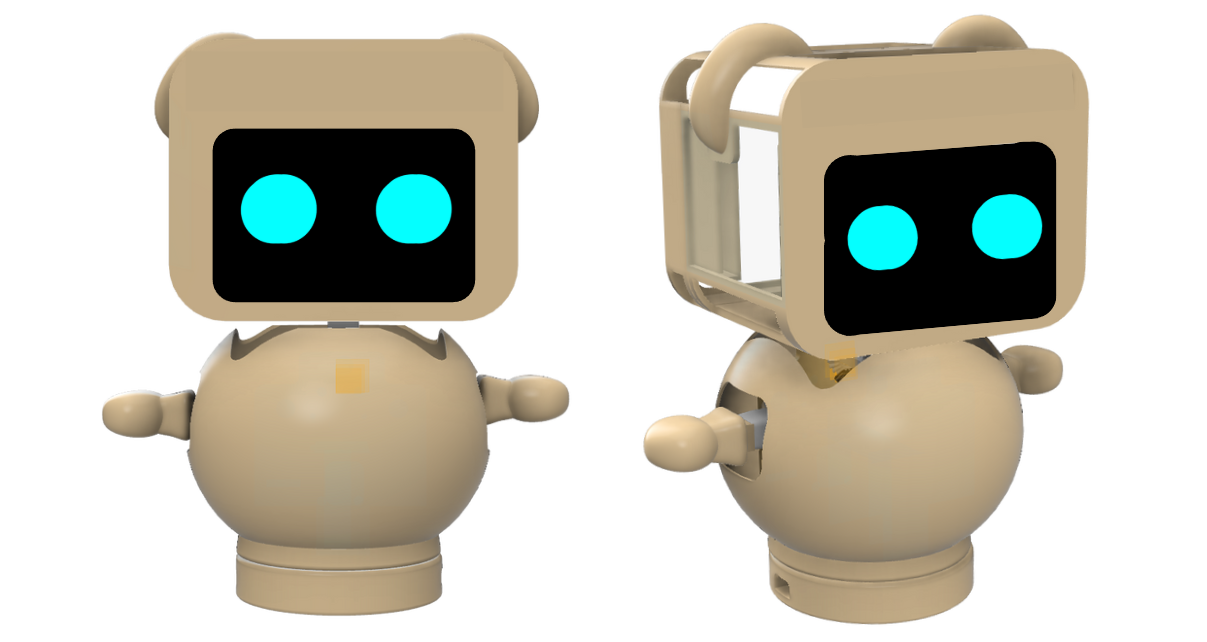
\includegraphics[width=\textwidth]{1-cad.png}
    \captionsetup{justification=centering}
    \caption{Pookie CAD Mockup}
    \label{fig:1-cad}
\end{figure}

In terms of design, Pookie’s physical design mockup is shown in Figure \ref{fig:1-cad}, consisting of three main components: the head, body, and base. The head was designed to resemble a baby bear, intended to evoke a sense of warmth and familiarity—almost as if the robot were a pet. Its eyes are represented by an LCD screen that displays various patterns to bring the robot to life. The spherical body houses key mechanical components, including motors that enable movement of the arms, head, and base. Finally, the base serves as Pookie’s foundation, containing essential electrical components such as the microcontroller and batteries.
\newpage
In terms of features, Pookie primarily does two tasks: analyze the user’s emotion and produce an output. Firstly, Pookie analyzes the user’s emotion by leveraging two channels, the user's face and speech. Utilizing data processing, statistics, and AI, Pookie attempts to understand what emotional state the user is at (e.g happy, sad, stressed, etc.). Secondly, after understanding the emotional state, Pookie produces an action through three modes: physical movement, eyes movement, and sound production. For instance, if the user is happy, then Pookie will attempt to maintain this happiness through moving excitedly or making funny noises. However, if the user is stressed, then Pookie will attempt to reduce these negative feelings by raising its hands trying to hug the user. The entire flow is summarized in Figure \ref{fig:2-flow}’s flowchart.

\begin{figure}[ht]
    \centering
    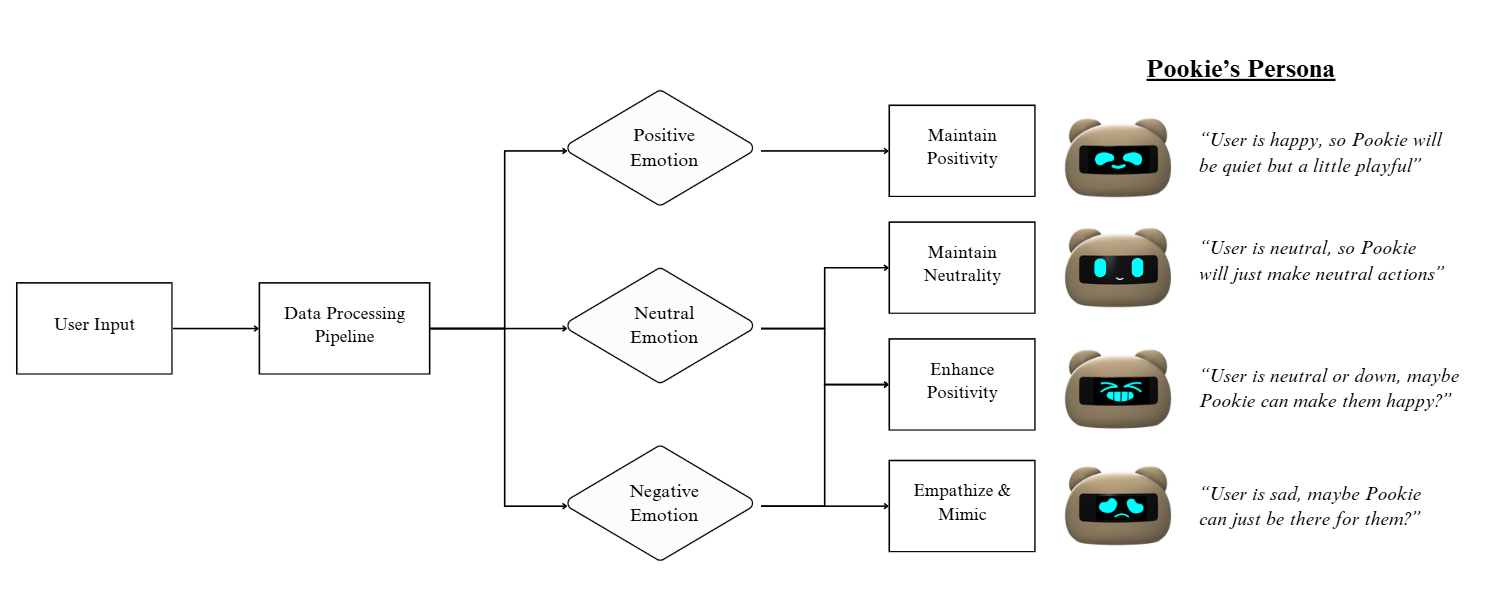
\includegraphics[width=\textwidth]{2-flow.png}
    \captionsetup{justification=centering}
    \caption{Pookie Action Flowchart}
    \label{fig:2-flow}
\end{figure}

Pookie brings together a friendly design and smart features to provide emotional support and comfort to users. It recognizes how a person feels by analyzing facial expressions and voice, then responds in a caring or playful way to match their emotional needs. With this foundation in place, the next section will summarize Pookie’s through two development stages: MVP 1 and MVP 2, carried out during the previous and current academic semesters.

\subsection{MVP 1 - Proof of Concept}
The first phase of the project is named “MVP 1 - Proof of Concept” and spanned the first academic semester. The purpose of this phase was to conduct research to validate the project, as well as build necessary foundations for the second phase. Key initiatives included validating the project concept using primary and secondary research methodologies. On the former side, the team spent three weeks conducting expert interviews with professional psychologists from Chula Student Wellness, a platform for free psychological counseling for Chula students. On the latter side, the team consolidated potential technologies to be used for the implementation of the project, such as potential models to be used for facial emotion recognition, and evaluated them under various factors. 

Overall, the phase came out as a success, with key three objectives fulfilled: designing the physical appearance, designing interactive features, and developing accurate emotion detection algorithms. These achievements lay a significant foundation for the rest of the objectives, where the team must continue building the essential components of the robot, and test under real circumstances. 

\subsection{MVP 2 - Functioning Prototype}
The second phase of the project is named “MVP 2 - Functioning Prototype” and spans the second academic semester. The purpose of this phase was to leverage the foundations established in the first phase, to develop and test the rest of the robot’s components. Key initiatives included enhancing the robot’s emotion detection algorithm, software and hardware integration, and user experience enhancement. Firstly, in terms of the emotion algorithm, the team leveraged Bayesian networks and decision trees to enhance the emotion detection logic. Secondly, regarding integration, the team worked on acquiring and building the hardware components of the robot, then integrating them with the software components to obtain a minimum functioning prototype.  Finally, user experience was enhanced through the use of wake-up words and other features to ensure seamlessness. 

However, given the time constraints and problems encountered throughout the project, the team could not achieve one objective: testing. Initially, the team aimed to test the robot through two methods: a controlled functionality test at MI Innovation Labs, and a long in-depth testing with a single user. Thus, the team focused on improving the user experience instead.
